%% Figure 1 (study design) as a standalone vector file: pdflatex Figure_1_source && rename to Figure_1.pdf
\documentclass[border=4pt]{standalone}
\usepackage[T1]{fontenc}
\usepackage{lmodern}
\usepackage{tikz}
\usetikzlibrary{arrows.meta}
\begin{document}
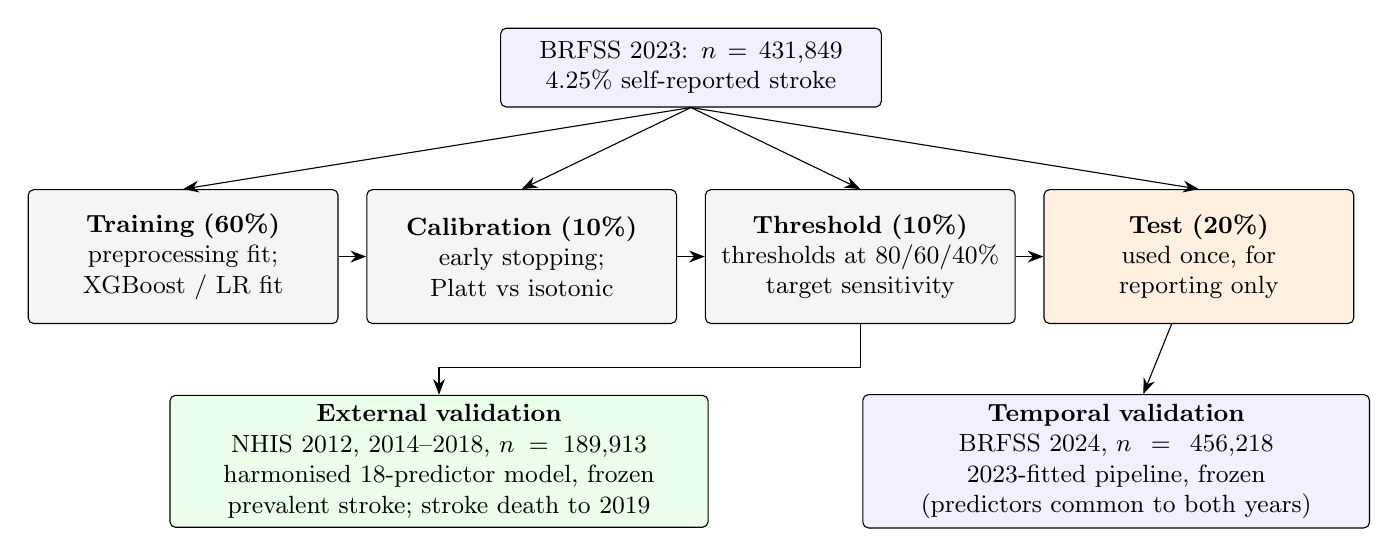
\begin{tikzpicture}[font=\small,
  box/.style={draw, rounded corners=2pt, align=center, minimum height=17mm, text width=37mm, fill=#1},
  box/.default=white, >={Stealth[length=2mm]}]
\node[box=blue!6, text width=46mm, minimum height=10mm] (data) at (0,0) {BRFSS 2023: $n=431{,}849$\\4.25\% self-reported stroke};
\node[box=gray!8] (tr) at (-6.45,-2.4) {\textbf{Training (60\%)}\\preprocessing fit;\\XGBoost / LR fit};
\node[box=gray!8] (ca) at (-2.15,-2.4) {\textbf{Calibration (10\%)}\\early stopping;\\Platt vs isotonic};
\node[box=gray!8] (th) at (2.15,-2.4) {\textbf{Threshold (10\%)}\\thresholds at 80/60/40\%\\target sensitivity};
\node[box=orange!12] (te) at (6.45,-2.4) {\textbf{Test (20\%)}\\used once, for\\reporting only};
\node[box=blue!6, text width=62mm, minimum height=10mm] (t24) at (5.4,-5.0) {\textbf{Temporal validation}\\BRFSS 2024, $n=456{,}218$\\2023-fitted pipeline, frozen\\(predictors common to both years)};
\node[box=green!8, text width=66mm, minimum height=10mm] (nh) at (-3.2,-5.0) {\textbf{External validation}\\NHIS 2012, 2014--2018, $n=189{,}913$\\harmonised 18-predictor model, frozen\\prevalent stroke; stroke death to 2019};
\foreach \n in {tr,ca,th,te} \draw[->] (data.south) -- (\n.north);
\draw[->] (tr) -- (ca); \draw[->] (ca) -- (th); \draw[->] (th) -- (te);
\draw[->] (te) -- (t24); \draw[->] (th.south) |- ++(0,-0.55) -| (nh.north);
\end{tikzpicture}
\end{document}
